 \documentclass[11pt]{beamer}
\usetheme{Warsaw}
\usepackage[utf8]{inputenc}
\usepackage{amsmath}
\usepackage{array}
\usepackage{amsfonts}
\usepackage{amssymb}
\usepackage{tikz}
\usetikzlibrary{arrows,automata}
%\usepackage[latin1]{inputenc}

\author{Team Expeditus}
\title{UAV Autonomous Landing}
%\setbeamercovered{transparent} 
%\setbeamertemplate{navigation symbols}{} 
%\logo{} 
\institute{SDSMT MCS} 
%\date{} 
%\subject{} 
\begin{document}

\begin{frame}
\titlepage
\end{frame}

%\begin{frame}
%\tableofcontents	
%\end{frame}

\begin{frame}{Introduction}
\textbf{UAV Autonomous Landing Project}\\
\vspace{12mm}
\textbf{Team Expeditus}\\
Jonathan Dixon, Dylan Geyer, Christopher Smith, Steven Huerta\\ 
\vspace{6mm}
\textbf{Sponsor}\\
Dr. Larry Pyeatt\\
\end{frame}


\begin{frame}{Goal}
Demonstrate the capability of a UAV to autonomously take-off, navigate through some waypoints, return to the landing pad, and land with a minimum of distance and orientation error. 
\end{frame}


\begin{frame}{Requirements}
\textbf{Goal}\\
\begin{itemize}
\item receive a set of waypoints
\item autonomously take-off
\item navigate through waypoints
\item return to launch pad
\item \textbf{land with $\pm$.1 distance and $\pm$15$^{\circ}$ orientation error}
\end{itemize}
\vspace{6mm}
\textbf{Limitations}\\
\begin{itemize}
\item landing platform is a fixed position
\item landing platform is a stable, horizontal surface
\item environment is ideal(no wind, gps available, no obstacles)
\end{itemize}
\end{frame}


\begin{frame}{User Stories/Backlog}

\begin{itemize}
\item \textbf{User 1(U-1):}\\ As a user, I want to communicate the waypoints to the UAV.
\item \textbf{Owner 1(O-1):}\\ As an owner, I want the UAV to autonomously take-off from the landing pad.
\item \textbf{Owner 2(O-2):}\\ As an owner, I want the UAV to autonomously navigate through a set of waypoints.
\item \textbf{Owner 3(O-3):}\\ As an owner, I want the UAV to autonomously return to the location of the landing pad.
\item \textbf{Owner 4(O-4):}\\ As an owner, I want the UAV to autonomously land on the landing pad without damaging the craft.
\item \textbf{Owner 5(O-5):}\\ As an owner, I want the UAV to autonomously land on the landing pad with the correct orientation.
\item \textbf{Common:}\\ Tasks relating to more than one user story(i.e. resolving dependencies).
\end{itemize}

\end{frame}

\begin{frame}{U-1}
\textbf{As a user, I want to communicate the waypoints to the UAV.}
\begin{tabular}{| c | >{\raggedright}m{4cm} | c | c |}\hline
Task No. & Task & Date Completed & Sprint\\\hline
1 & Review previous method/interface for communicating coordinates to UAV. & 10/05/15 & 1 \\\hline
2 & Review code that communicates with quadrotor & 10/16/15 & 2 \\\hline
3 & Review code that allows a user to input waypoints & 10/16/15 & 2\\\hline

\end{tabular}
\end{frame}


\begin{frame}{O-1}
\textbf{As an owner, I want the UAV to autonomously take-off from the landing pad.}
\begin{tabular}{| c | >{\raggedright}m{4cm} | c | c |}\hline
Task No. & Task & Date Completed & Sprint\\\hline
1 & Review previous implementation for autonomous take-off. & 10/05/15 & 1 \\\hline
2 & Review code that enables the quadrotor to autonomously take-off from landing pad & 10/16/15 & 2 \\\hline

\end{tabular}
\end{frame}


\begin{frame}{O-2}
\textbf{As an owner, I want the UAV to autonomously navigate through a set of waypoints.}
\begin{tabular}{| c | >{\raggedright}m{4cm} | c | c |}\hline
Task No. & Task & Date Completed & Sprint\\\hline
1 & Review previous implementation for navigating waypoints. & 10/05/15 & 1 \\\hline
2 & Review code that enables the quadrotor to autonomously navigate through a series of way-points & 10/16/15 & 2 \\\hline

\end{tabular}
\end{frame}


\begin{frame}{O-3}
\textbf{As an owner, I want the UAV to autonomously return to the location of the landing pad.}
\begin{tabular}{| c | >{\raggedright}m{4cm} | c | c |}\hline
Task No. & Task & Date Completed & Sprint\\\hline
1 & Review previous implementation to autonomously return to location of landing pad & 10/05/15 & 1 \\\hline
2 & Review code that allows the autonomous return of the UAV to the landing pad. & 10/16/15 & 2 \\\hline

\end{tabular}
\end{frame}


\begin{frame}{O-4}
\textbf{As an owner, I want the UAV to autonomously land on the landing pad without damaging the craft}
\begin{tabular}{| c | >{\raggedright}m{4cm} | c | c |}\hline
Task No. & Task & Date Completed & Sprint\\\hline
1 & Review previous implementation for autonomous landing & 10/05/15 & 1 \\\hline
2 & Install previous implementation & 10/19/15 & 2 \\\hline
3 & Test previous implementation & 10/26/15 & 2\\\hline

\end{tabular}
\end{frame}


\begin{frame}{O-5}
\textbf{As an owner, I want the UAV to autonomously land on the landing pad with the correct orientation.}
\begin{tabular}{| c | >{\raggedright}m{4cm} | c | c |}\hline
Task No. & Task & Date Completed & Sprint\\\hline
1 & Review previous implementation for autonomous landing & 10/05/15 & 1 \\\hline
2 & Install previous implementation & 10/19/15 & 2 \\\hline
3 & Test previous implementation & 10/26/15 & 2\\\hline
\end{tabular}
\end{frame}


\begin{frame}{C}
\textbf{Initial Common Tasks}
\begin{tabular}{| c | >{\raggedright}m{4cm} | c | c |}\hline
Task No. & Task & Date Completed & Sprint\\\hline
1 & Install Ubuntu 14.04 or some other ROS Indigo/Jade distro compliant OS. & 09/25/15 & 1 \\\hline
2 & Setup Gazebo 6.+ & 09/25/15 & 1 \\\hline
3 & Download Rviz package & 09/25/15 & 1\\\hline
4 & Setup Simulation Environment & 11/02/15 & 2 \\\hline
\end{tabular}
\end{frame}


\begin{frame}{C Continued}
\textbf{Initial Common Tasks}
\begin{tabular}{| c | >{\raggedright}m{4cm} | c | c |}\hline
Task No. & Task & Date Completed & Sprint\\\hline
5 & Review previous iteration of project documentation & 09/25/15 & 1 \\\hline
6 & Inspect current quadrotor configuration & 09/28/2015 & 2\\\hline
7 & Identify parts needed for quadrotor & 11/02/2015 & 2 \\\hline
8 & Acquire parts needed for hexrotor & 12/01/2015 & 3 \\\hline
\end{tabular}
\end{frame}

%%% End SECTION 1 


%% Begin SECTION 2 
\begin{frame}{Design}
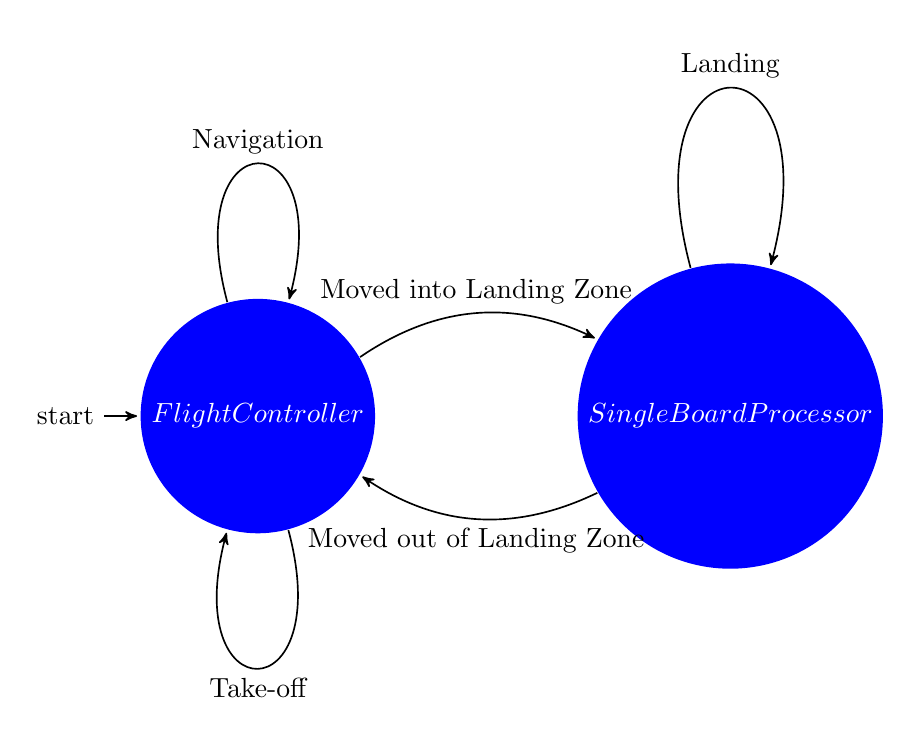
\begin{tikzpicture}[->,>=stealth',shorten >=1pt,auto,node distance=6cm,
                    semithick]
  \tikzstyle{every state}=[fill=blue,draw=none,text=white]

  \node[initial,state] (A)              {$Flight Controller$};
  \node[state]         (B) [right of=A] {$Single Board Processor$};

  \path (A) edge [loop below] node {Take-off} (A)
            edge [loop above]  node {Navigation} (A)
            edge [anchor=center,bend left,above] node {Moved into Landing Zone} (B)
        (B) edge [loop above] node {Landing} (B)
            edge [anchor=center,bend left,left,below]  node {Moved out of Landing Zone} (A);
\end{tikzpicture}
\end{frame}

\begin{frame}{Architecture}
\begin{figure}
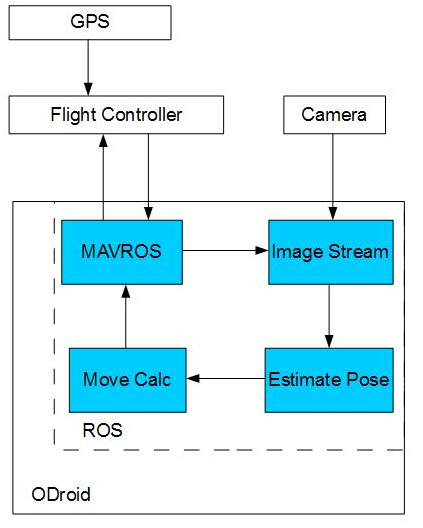
\includegraphics[width=.5\textwidth]{images/broad_approach1}
\end{figure}

\end{frame}

\begin{frame}{Hardware Requirements}
\begin{itemize}
\item ODroid XU4
\item Pixhawk Flight Controller
\item GPS peripheral
\item Camera
\item Battery
\item UAV(Frame, Motors, ESCs, Power Distribution Board)
\end{itemize}

\end{frame}

\begin{frame}{Software Requirements}
\begin{itemize}
\item Mavlink
\item OpenCV
\item Robot Operating System(ROS) Indigo/Jade Distro
\item Ubuntu 14.04
\end{itemize}

\end{frame}



% Include Architecture/Design/Tech Specs/& Tools ---Likely will take a few slides 
\begin{frame}{UAV Design \& Tech Specs}

\end{frame}

% Include Architecture/Design/Tech Specs/& Tools ---Likely will take a few slides 
\begin{frame}{Visual Homography Design \& Tech Specs}

\end{frame}

% Include Architecture/Design/Tech Specs/& Tools ---Likely will take a few slides 
\begin{frame}{Simulation Design \& Tech Specs}

\end{frame}

%% END SECTION 2


%% BEGIN SECTION 3
\begin{frame}{Testing}
PLACE HOLDER FOR THIS STUFF:
Unit or Component Testing,  System Testing,  System Integration,  Remaining backlog,  Revised goals
and Revised Deliverable
\end{frame}

% How are we going to test the UAV 
\begin{frame}{UAV Testing}

Manual Flight \\
Autonomous Flight \\

\end{frame}

% How are we going to test the VH Landing Algorithm
% Maybe discuss tests at the different stages (blob color recog, dist/dir output, real-time output (How many frames?)) 
\begin{frame}{Visual Homography Landing Testing}

\end{frame}

% How do we plan to integrate the different systems together
\begin{frame}{Integration}

\end{frame}


\begin{frame}{Remaining Backlog}
\begin{itemize}
\item \textbf{User 1(U-1)}
\item \textbf{Owner 1(O-1)}
\item \textbf{Owner 2(O-2)}
\item \textbf{Owner 3(O-3)}
\item \textbf{Owner 4(O-4)}
\item \textbf{Owner 5(O-5)}
\item \textbf{Common}
\end{itemize}

\end{frame}


\begin{frame}{Revised Goals}

Project Goals remain fixed

\end{frame}


%% END SECTION 3


%% BEGIN SECTION 4
\begin{frame}{Successes and Issues}
PLACE HOLDER FOR THIS STUFF:
Successes (goals met), Issues or problems (goals not met), Risk Analysis, Risk Mitigation, Timeline,
Budget/costs, Intellectual Property Aspects, Licensing
\end{frame}

\begin{frame}{Successes}

Parts are now in!!\\



\end{frame}

\begin{frame}{Issues}

\begin{itemize}
\item \textbf{Simulation:}\\
\begin{itemize}
\item Prevents testing landing algorithms safely(O-5,O-6)
\end{itemize}
\item \textbf{Waiting for Parts:}\\
\begin{itemize}
\item Prevents HIL Alternative
\item Prevents UAV Manual Flight(C)
\item Prevents UAV Autonomous Flight(U-1,O-1,O-2,O-3)
\end{itemize}
\item \textbf{VH Landing Algorithm:}\\
\end{itemize}

\end{frame}

\begin{frame}{Risk Analysis}
\begin{itemize}
\item Simulation: SITL has proven to be problematic
\item UAV Build: Borrowing items from UAV Team (Radio and Control)
\item UAV Build: One UAV for physical testing and demonstration
\item Landing Algorithm: ???
\end{itemize}


\end{frame}

\begin{frame}{Risk Mitigation}
\begin{itemize}
\item Simulation:
\begin{itemize}
\item Attempt HIL as Alternative
\end{itemize}

\item UAV Build(Sharing)
\begin{itemize}
\item Schedule use of tools to prevent conflict
\item Request more funding if schedule is untenable
\end{itemize}

\item UAV Build(One Shot)
\begin{itemize}
\item Integrate manual control override
\item Validate solutions through simulation
\end{itemize}

\end{itemize}
\end{frame}


\begin{frame}{Timeline}
\textbf{Sprint 3.5 12/16/15 to 1/10/16}
\begin{itemize}
\item Finish UAV Build(C)
\item Manual Flight of UAV(C)
\item Autonomous Flight of UAV(C,U-1,O-1,O-2,O-3)
\item Resolve Simulation Issues(C)
\end{itemize}
\vspace{2mm}
At the end of break, 3 backlog items will have been completed\\
\vspace{4mm}
\textbf{Sprint 4 1/18/16~2/5/16}
\begin{itemize}
\item Finish Landing Algorithm Simulations(O-4,O-5)
\end{itemize}
\vspace{2mm}
At the end of sprint 4, we should have a landing approach validated by simulation.
\end{frame}


\begin{frame}{Timeline...continued}
\textbf{Sprint 5 2/15/16~3/4/16}
\begin{itemize}
\item Integration of Landing Autonomy on UAV(O-4,O-5)
\end{itemize}
\vspace{2mm}
At the end of sprint 5, we should have completed the remainder of backlog items.\\
\vspace{4mm}
\textbf{Sprint 6 3/21/16~4/15/16}
\begin{itemize}
\item Refinement
\end{itemize}
\vspace{2mm}
At the end of sprint 6, project will be complete
\end{frame}

\begin{frame}{Budget}
\begin{table}[]
\centering
\begin{tabular}{|l|l|l|l|}
\hline
Item               & Qty & Price    & Total    \\ \hline
                   &     &          &          \\ \hline
Frame              & 1   & \$79.99  & \$79.99  \\ \hline
Motors             & 8   & \$23.99  & \$191.92 \\ \hline
ESCs               & 8   & \$17.78  & \$142.24 \\ \hline
Pixhawk            & 1   & \$199.99 & \$199.99 \\ \hline
Power Distribution & 1   & \$19.99  & \$19.99  \\ \hline
GPS Mast           & 2   & \$10.00  & \$20.00  \\ \hline
GPS                & 2   & \$89.99  & \$179.98 \\ \hline
Power Module       & 1   & \$24.99  & \$24.99  \\ \hline
Odroid XU4         & 1   & \$75.95  & \$75.95  \\ \hline
Props(set of 4)    & 3   & \$7.55   & \$22.65  \\ \hline
                   &     &          &          \\ \hline
TOTAL              &     &          & \$957.70 \\ \hline
\end{tabular}
\end{table}


\end{frame}


\begin{frame}{IP \& Licensing}
Intellectual Property:\\
Project is owned by SDSMT\\
\vspace{4mm}
Licensing for Dependencies:
\begin{itemize}
\item OpenCV: BSD 
\item ROS: BSD
\item Mavlink: LGPL
\item QGroundControl: GPL
\end{itemize}


\end{frame}

%% END SECTION 4


%% BEGIN SECTION 5
\begin{frame}{Prototypes and Demos}
PLACE HOLDER FOR THIS STUFF:
Demos!!
\end{frame}

\begin{frame}{Simulation - PX4 ROS SITL}
\begin{figure}
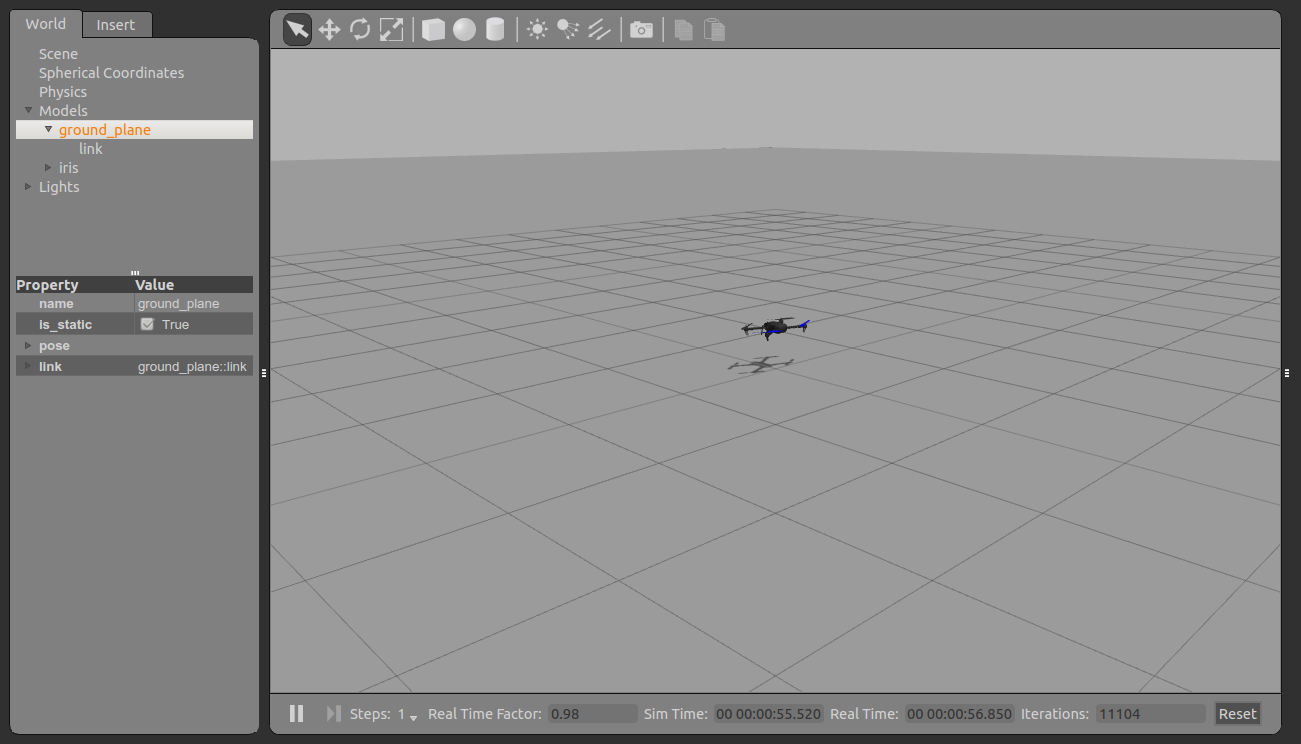
\includegraphics[width=1\textwidth]{images/flight1}
\end{figure}
\end{frame}

\begin{frame}{PX4 ROS SITL...continued}
\begin{figure}
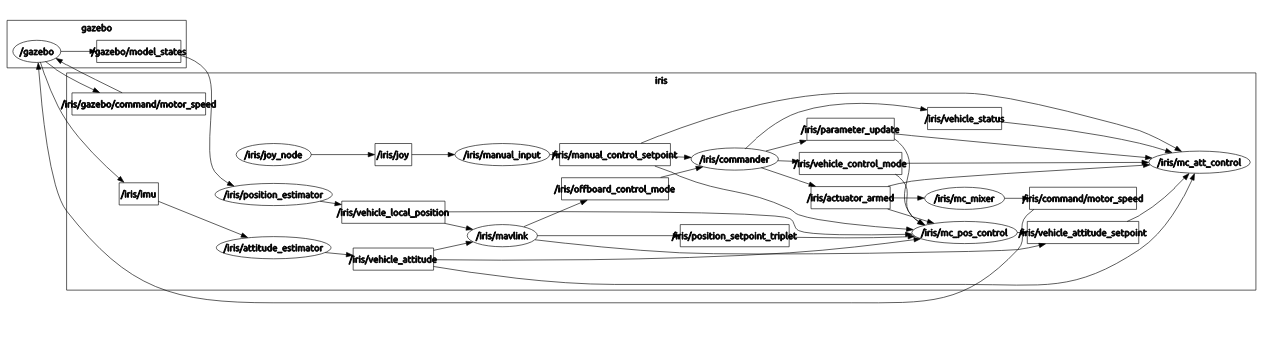
\includegraphics[width=1\textwidth]{images/px4graph}
\end{figure}
\end{frame}

\begin{frame}{PX4 ROS SITL...continued}
\begin{figure}
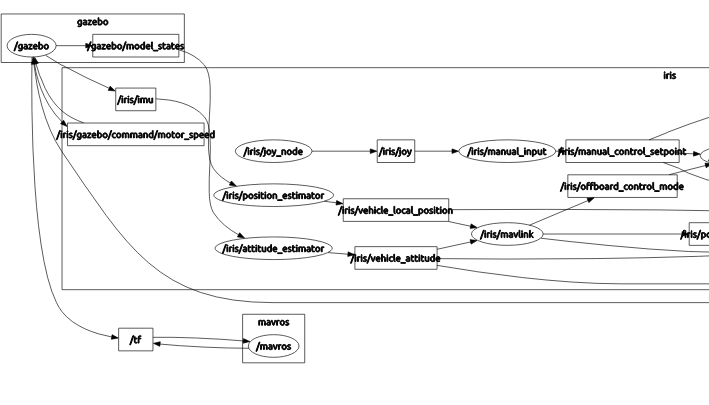
\includegraphics[width=1\textwidth]{images/mavros_sitl}
\end{figure}
\end{frame}

\begin{frame}{PX4 ROS SITL...continued}
\begin{figure}
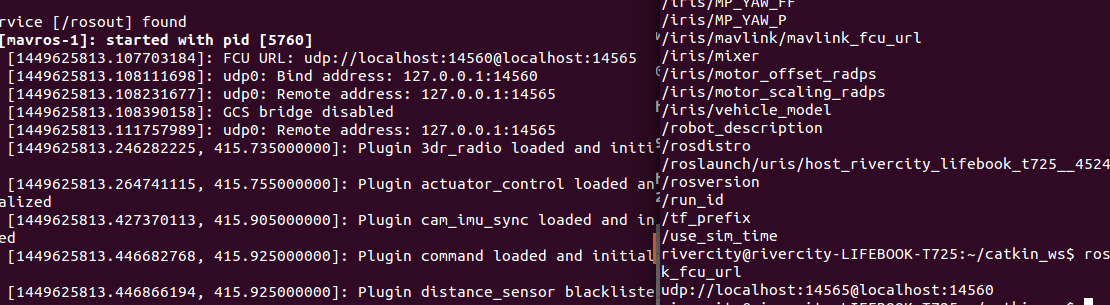
\includegraphics[width=1\textwidth]{images/params}
\end{figure}
\end{frame}

\begin{frame}{Ground Control Station - QGroundControl}
\begin{figure}
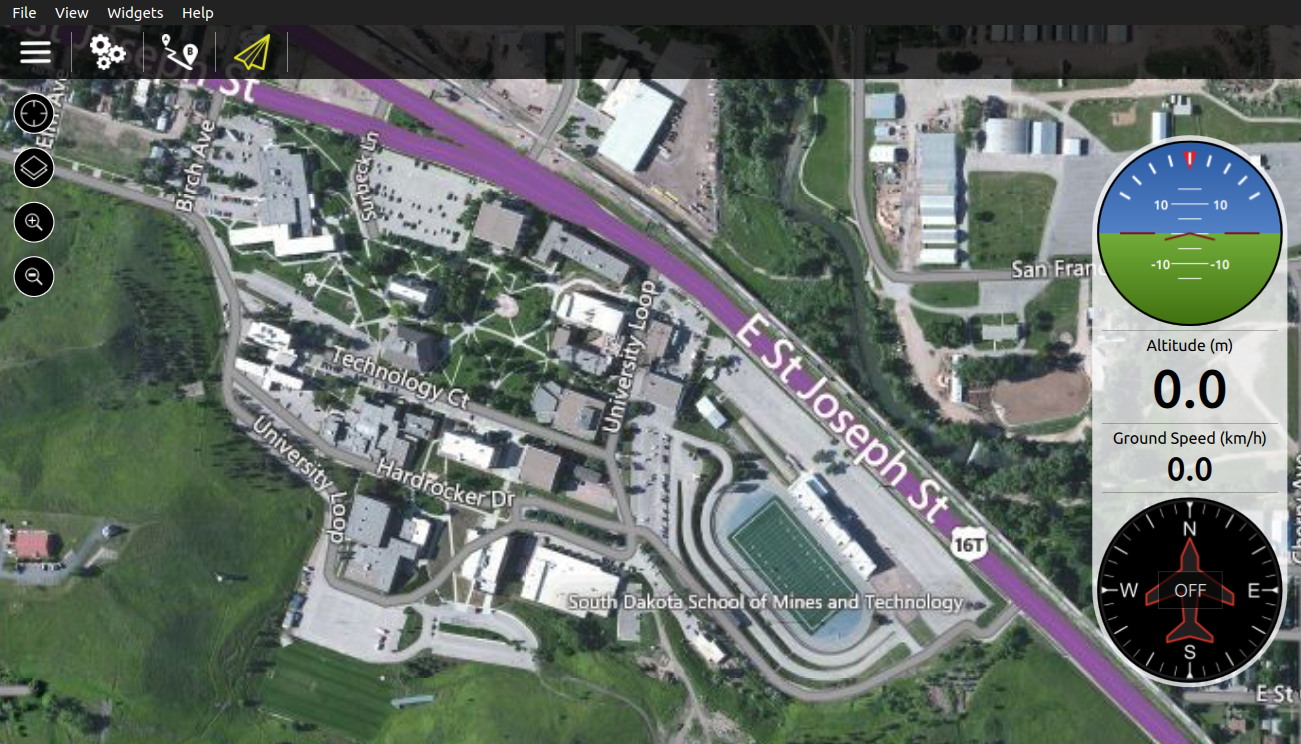
\includegraphics[width=1\textwidth]{images/qgroundcontrol}
\end{figure}
\end{frame}

\begin{frame}{Ground Control Station...continued}
\begin{figure}
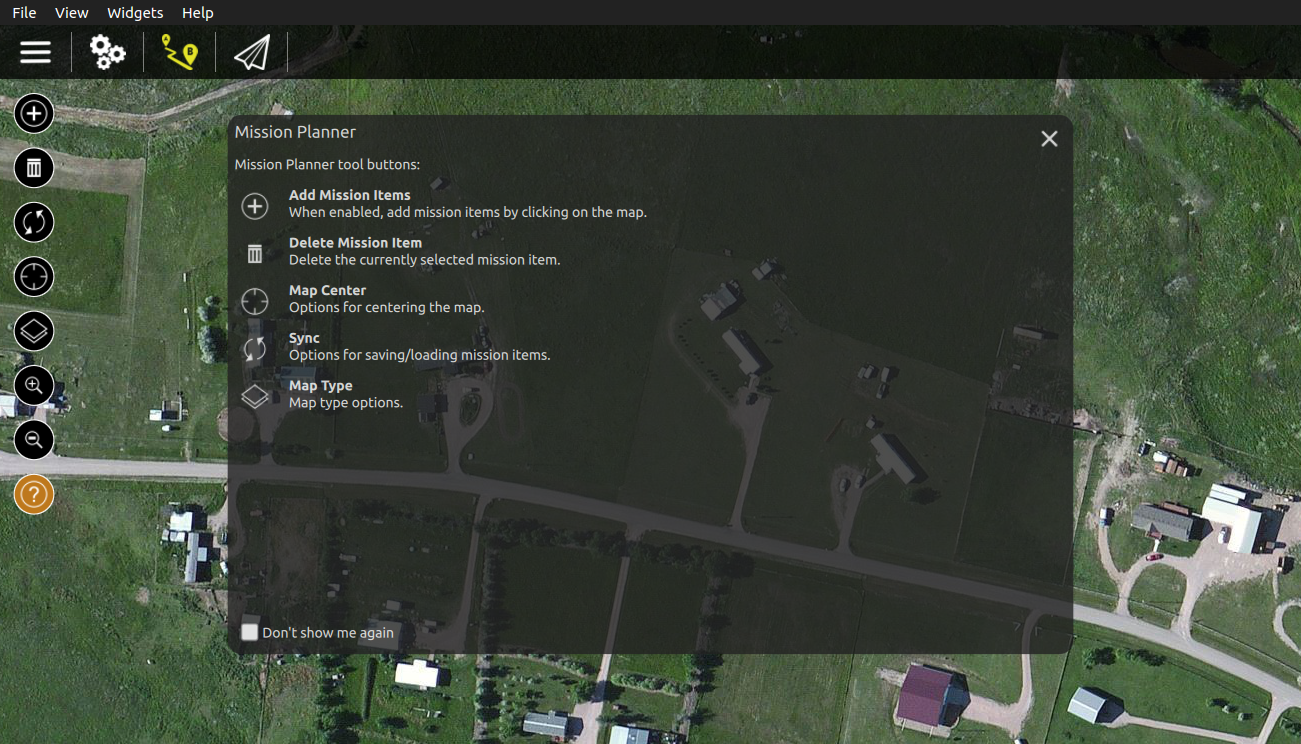
\includegraphics[width=1\textwidth]{images/selectmission}
\end{figure}
\end{frame}

\begin{frame}{Ground Control Station...continued}
\begin{figure}
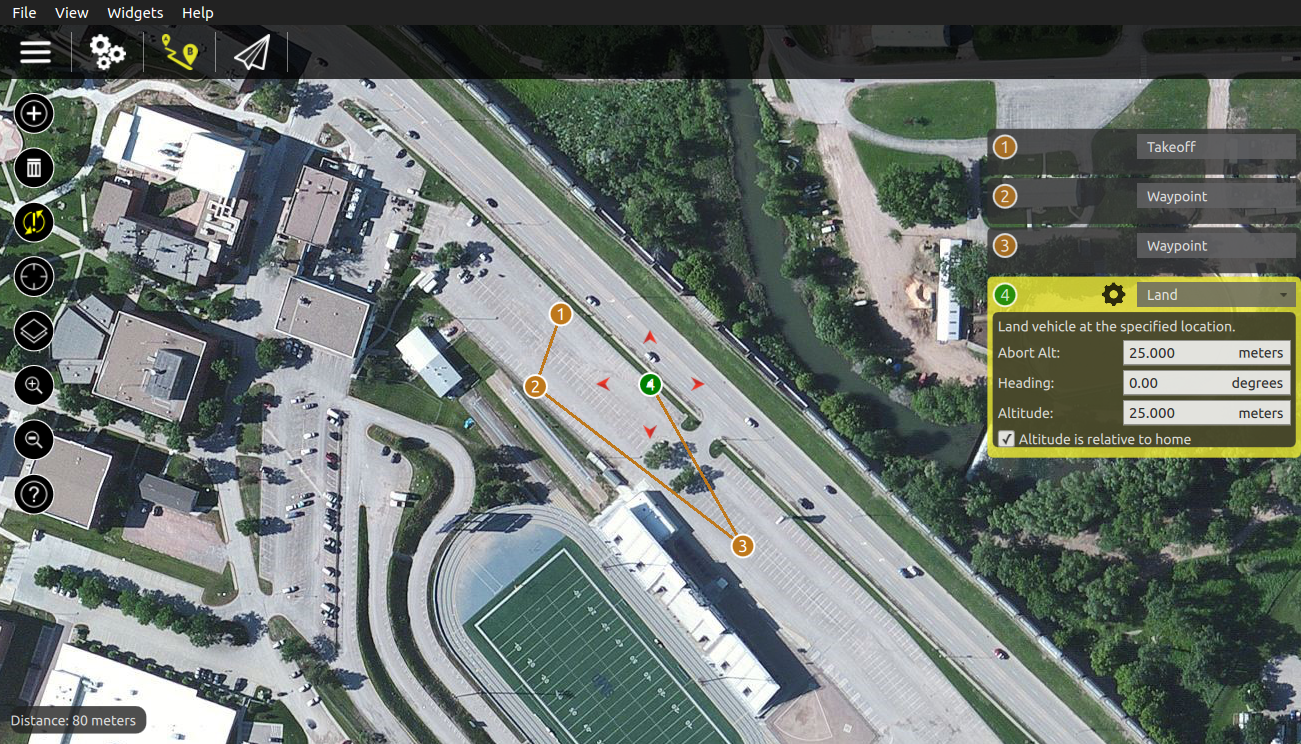
\includegraphics[width=1\textwidth]{images/mission}
\end{figure}
\end{frame}

%% END SECTION 5
\begin{frame}{ END}
\end{frame}



\end{document}
